\documentclass[12pt, a4paper]{article}
\usepackage[utf8]{inputenc}
\usepackage{graphicx}
\usepackage[portuguese]{babel}
\usepackage{amsmath, amssymb}
\usepackage[hidelinks]{hyperref}
\usepackage{geometry}
\geometry{margin=1in}

\title{Trabalho final de Computação Reconfigurável}
\author{Alexandre André Neves Pita\\
Instituto Superior de Engenharia \\
Universidade do Algarve \\}
\date{\today}

\begin{document}

\begin{titlepage}
    \centering
    \vspace*{2cm}

    {\Large\textbf{Universidade do Algarve}}\\[1.5cm]

    {\Huge\textbf{Trabalho final de Computação Reconfigurável}}\\[2cm]

    {\Large Alexandre André Neves Pita}\\
    74526\\[1.5cm]

    {\large Curso de Engenharia de Sistemas e Tecnologicas Informáticas}\\
    Instituto Superior de Engenharia\\[2cm]

    {\large \today}

    \vfill
\end{titlepage}
\pagenumbering{roman} % Use Roman numerals for TOC and front matter
\newpage
\tableofcontents
\newpage

\pagenumbering{arabic} % Switch to normal numbering

\section{Introdução}
O Trabalho Final da unidade curricular de Computação Reconfigurável tem como principal objetivo o desenvolvimento de um projeto que integre diversos componentes de hardware reconfigurável,
 implementados em VHDL, os quais foram previamente concebidos ao longo dos trabalhos realizados durante o semestre.
Este projeto pretende consolidar os conhecimentos adquiridos, promovendo a aplicação prática dos mesmos, e explorar a interligação e o controlo conjunto de vários módulos.\\
\\
O procedimento deste trabalho consiste na filtragem de um sinal com ruído, com o objetivo de obter um sinal mais limpo.\\  
Antes de ser transmitida, a informação proveniente do filtro é processada por um módulo de encriptação, que assegura a proteção dos dados durante a transmissão.\\
De seguida, a informação encriptada é enviada para um módulo UART, responsável pela transmissão em série para o "Controller2".\\
No "Controller2", essa mesma informação é recebida por outro módulo UART, que converte os dados de formato série para paralelo, permitindo o seu encaminhamento para o módulo de desencriptação.\\
Após o processo de desencriptação, procede-se à filtragem do sinal, sendo os dados resultantes armazenados num ficheiro ROM.\\


A imagem apresentada em seguida ilustra a arquitetura simplificada do sistema proposto para este trabalho.\\

\begin{figure}[h]  % 'h' means "here" (placement)
    \centering
    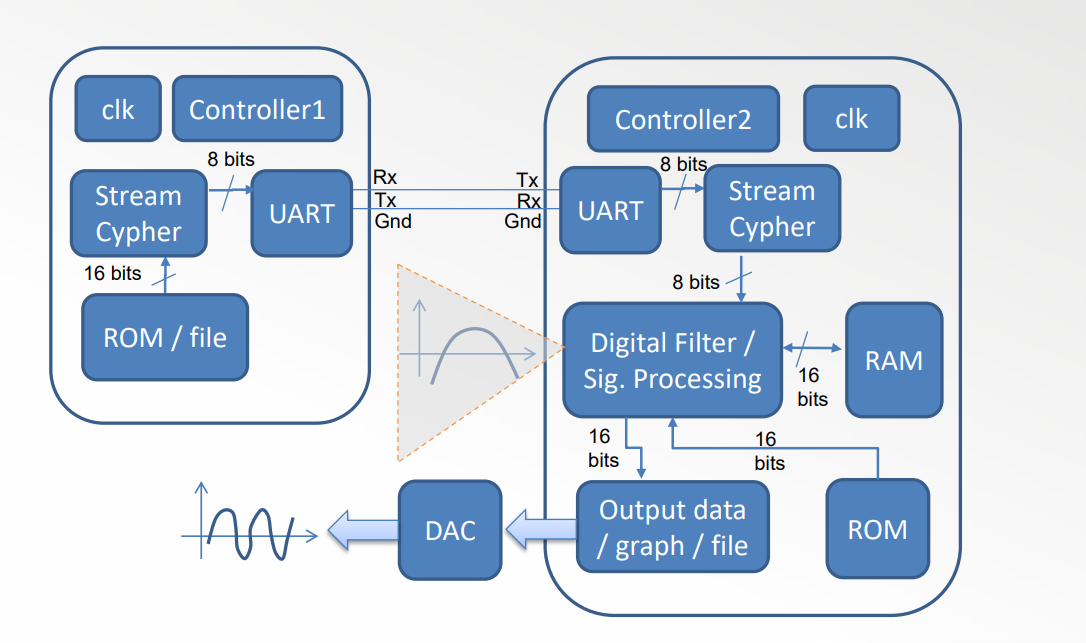
\includegraphics[width=0.6\textwidth]{./images/architecture.png}  % adjust width or use height=
    \caption{Arquitetura do sistema proposto.}
    \label{fig:arquitetura}
\end{figure}

Ao observar a imagem, é possível identificar dois controladores, designadamente o "Controller1" e o "Controller2". \\ 
No interior do "Controller1" encontram-se vários módulos, descritos na lista abaixo:

\begin{itemize}
    \item \textbf{Módulo ROM / File:} Módulo que contém informação acessível por outros componentes.  
    Neste projeto, foi utilizada uma ROM para armazenamento dos dados correspondentes ao filtro.
    
    \item \textbf{Módulo Cypher:} Responsável pela encriptação da mensagem proveniente da ROM.
    
    \item \textbf{Módulo UART:} Encarregado de transmitir, de forma sequencial, a informação encriptada para o "Controller2".
\end{itemize}


No "Controller2", também existem vários módulos, que são os seguintes:

\begin{itemize}
    \item \textbf{Módulo UART:} Encarregado de receber, de forma sequencial, a informação encriptada pelo "Controller1".

    \item \textbf{Módulo Cypher:} Responsável pela desencriptação da mensagem proveniente da ROM.
    \item \textbf{Módulo Digital Filter:} Módulo responsável pela filtragem do sinal, que é processado pelo módulo de desencriptação.\\

    \item \textbf{Módulo ROM / File:} Módulo que contém informação acessível por outros componentes.  
    Neste projeto, foi utilizada uma ROM para armazenamento dos dados correspondentes ao sinal com ruído.

    \item \textbf{Módulo RAM:} RAM compoenente de escrita e leitura de dados. Neste projeto o mesmo não foi utilizado pois este foi escrito automáticamente para o ficheiro ROM.\\

    \item \textbf{Módulo Output data:} Escrita num ficheiro de texto, com o objetivo de armazenar os dados filtrados.\\
    
\end{itemize}

\newpage

\section{Literature Review}
Summarize relevant background and previous work.
\newpage

\section{Methodology}
Explain how you conducted the study or research.
\newpage

\section{Results and Discussion}
Present and interpret your findings.
\newpage

\section{Conclusion}
Summarize contributions and suggest future work.
\newpage

\bibliographystyle{plain}
\bibliography{references}  % Create a file named references.bib

\appendix
\section{Appendix A}
Any supplementary material here.

\end{document}